%%
%% 研究報告用スイッチ
%% [techrep]
%%
%% 欧文表記無しのスイッチ(etitle,jkeyword,eabstract,ekeywordは任意)
%% [noauthor]
%%

\documentclass[submit,techrep]{ipsj}
%\documentclass[submit,techrep,noauthor]{ipsj}



\usepackage[dvips]{graphicx}
\usepackage{latexsym}

\def\Underline{\setbox0\hbox\bgroup\let\\\endUnderline}
\def\endUnderline{\vphantom{y}\egroup\smash{\underline{\box0}}\\}
\def\|{\verb|}

\setcounter{巻数}{53}%vol53=2012
\setcounter{号数}{10}
\setcounter{page}{1}


\begin{document}


\title{無意識参加型センシングシステムの有効性の検証}

\etitle{Verification of the effectiveness of an Unconscious Participatory Sensing System}

%\affiliate{IPSJ}{情報処理学会\\
%IPSJ, Chiyoda, Tokyo 101--0062, Japan}


%\paffiliate{JU}{情報処理大学\\
%Johoshori Uniersity}

\affiliate{GSBACSA}{愛知工業大学大学院 経営情報科学研究科\\
Graduate School of Business Administration and Computer Science, Aichi Institute of Technology}
\affiliate{FISA}{愛知工業大学 情報科学部\\Faculty of Information Science, Aichi Institute of Technolog}
\affiliate{NTTDOCOMO}{NTTドコモ先進技術研究所\\Research Laboratories, NTT DOCOMO, Inc.}

\author{水上 貴晶}{Takamasa Mizukami}{GSBACSA}[b14723bb@aitech.ac.jp]
\author{堀 将之}{Masayuki Hori}{FISA}%[hori@pluslab.org]
\author{古謝 佑次}{Yuji Koja}{FISA}%[hori@pluslab.org]
%\author{大村 和徳}{Kazunori Omura}{FISA}[oremura@gmail.com]
%\author{河合 亮太}{Ryota Kawai}{FISA}
%\author{河南 光}{Hikaru Kawanami}{FISA}
\author{土井 千章}{Chiaki Doi}{NTTDOCOMO}%[chiaki.doi.tf@nttdocomo.com]
\author{太田 賢}{Ken Ohta}{NTTDOCOMO}%[ootaken@nttdocomo.com]
\author{稲村 浩}{Hiroshi Inamura}{NTTDOCOMO}%[inamura@nttdocomo.com]
\author{梶 克彦}{Katsuhiko Kaji}{FISA}%[kaji@aitech.ac.jp]
\author{内藤 克浩}{Katsuhiro Naito}{FISA}%[naito@pluslab.org]
\author{菱田 隆彰}{Takaaki Hishida}{FISA}%[hishida@aitech.ac.jp]
\author{水野 忠則}{Tadanori Mizuno}{FISA}%[mizuno@mizulab.net]


\begin{abstract}
detailを修正しました
スマートフォンの普及を背景に,一般ユーザの持つスマートフォンを利用して高密度,広範囲の環境情報を収集する参加型センシングの実現が期待をされている.しかし,参加型センシングは多くの参加者が存在する事を前提としており,実用的なシステムを構築するためには手軽に参加してもらい,より多くの参加者が必要である.
著者らは参加者にセンシング意識させない無意識参加型センシングの手法とプロトタイプ実装を行ってきた.
本稿では,従来の参加型センシングと無意識参加型センシングのシミュレータを構築し,センサデバイスが定点観測しているセンサデータの報告数を定量的に評価した.愛知工業大学をモデルとした参加者を自由に動かしたシナリオにおいてセンサデバイスと参加者の持つスマートフォンとで無線通信を行いデータ取得を実現した.シミュレーションの結果,無意識参加型センシングの特性と検証結果を報告する.
aaaaaaaaa
コードレビューで修正内容を修正したよ
コメント機能を追加してみた
コミュニティ一覧の作成開始
コミュニティ作成機能作成開始
\end{abstract}

ストーリー
無意識の必要性を記述(参加型センシングと比較)
無意識参加型センシングの概要
	想定環境
事前実験
シミュレーション評価
まとめ

章立て
はじめに
関連研究
無意識参加型センシングの概要
	想定環境
事前実験
シミュレーション評価
まとめ



\begin{jkeyword}
情報処理学会論文誌ジャーナル,\LaTeX,スタイルファイル,べからず集
\end{jkeyword}

\begin{eabstract}
This document is a guide to prepare a draft for submitting to IPSJ
Journal, and the final camera-ready manuscript of a paper to appear in
IPSJ Journal, using {\LaTeX} and special style files.  Since this
document itself is produced with the style files, it will help you to
refer its source file which is distributed with the style files.
\end{eabstract}

\begin{ekeyword}
IPSJ Journal, \LaTeX, style files, ``Dos and Dont's'' list
\end{ekeyword}

\maketitle

%1
\section{はじめに}

%研究背景を記述
%参考文献を引用しながら述べる

近年,安価で高精度な物理センサの普及によりセンサネットワークにおける研究が盛んに行われている.センサネットワークは様々な情報を収集するネットワークシステムとして着目されている\cite{Viani}.物理センサにより温度や湿度,照度などの環境情報を定量的に取得する事が可能である.また,スマートフォンの普及によって一般者が携帯するスマートフォンを用いたセンシングに着目されている.スマートフォンには加速度センサやGPSセンサなど様々な物理センサが搭載されている.そこでセンシングデバイスとしてスマートフォンを活用した参加型センシングに関する研究が行われている\cite{Nicholas}.

対象とする参加型センシングでは,センシングの依頼者が街中に散らばるスマートフォンを持つ参加者(一般者)に対して,センシングしたい各地点にセンシングを依頼するものと想定している\cite{Burke}.従って,前提条件としてセンシングをしたい各地点にセンシング参加者が多数存在している事である.センシング処理に一般者が関与することから,測定場所,測定対象,測定方法などの自由度が大きく,一般者の持つスマートフォンを用いた新たな情報収集手法として注目されている.


参加型センシングで収集する情報は大別して,人による評価情報を収集する場合\cite{Lam}と物理センサなどを用いて定量的に測定可能な事象を収集する場合\cite{Shinohara}がある.人による評価情報とは物理センサでは測定できない,人間の持つ五感を活かした主観的かつ定性的な情報を収集し従来のセンシングでは取得できなかった情報を広範囲,高密度なセンシング期待されている.一方,物理センサを用いた定量的に測定可能な事象を対象とした場合,参加者のスマートフォンに搭載されているセンサを利用する場合する事となる.そのため,システムから依頼を受けた参加者は,測定対象場所に移動しスマートフォンに搭載されているセンサ情報を取得する事になる.
しかし,現実的なセンシングを考えた場合,スマートフォンに搭載されている,温度,気圧などのセンサは,スマートフォンの機種が異なる場合やモデルによって,実装されているセンサが異なり,センサ情報の精度及び実装環境が異なる事が予測される.このような条件では,同一環境において測定を行ったとしても,スマートフォンの機種やモデルにより異なる測定値が得られる事が考えられる.そのため,スマートフォン内臓センサで利用可能なものは,加速度やGPSなどの比較的,機種やモデルの違いに影響を受けない測定値に限定されると予測される.結果として,特定の環境を継続的に測定する場合には,スマートフォンを通信回線として利用する一方で,測定自体は別デバイスを用いて測定値の精度を高める必要がある\cite{Li}.本稿では物理センサを用いた定量的に測定可能な事象を対象とした参加型センシングについて取り上げる.


参加型センシングにおいては参加者が自主的にセンシング処理に関与する必要があるため,多くの研究において参加者が積極的にセンシング処理に関与するための動機付け手法が検討されている\cite{Yoshitaka}.


また,参加型センシングとソーシャルメディアの情報を複合的に処理を行う手法なども提案されている\cite{Demirbas}.前述した通り,様々な研究が続けられているが,現状の参加型センシングでは,一般者を想定したシステムとまでは確立できておらず,センシングに興味を持つ一部の一般者を想定としている状況である.

本稿では,著者らが先行研究\cite{Mizukami}で行っている無意識参加型センシングをシミュレータScenargie\cite{Scenargie}を用いて,従来の参加型センシングとこれまでに提案してきた無意識参加型センシングのモデルを評価した.シミュレーションでは都市部を想定したシナリオを用いて,参加型センシングによるセンサデータ収集量と無意識参加型センシングによるデータ報告数を比較した結果,無意識参加型センシングにおいて,人通りの多い場所付近でのセンシングポイントにてセンシングデータをより多く収集できる事を確認できた.



情報処理学会では,基幹論文誌として論文誌ジャーナルの発行を行っている.こ
れまで論文誌ジャーナル編集委員会では,論文誌ジャーナルの論文掲載時のフォー
マット


これに伴い,\LaTeX のスタイルファイルも新しいものに変更した.本稿では,
まずそのスタイルファイルを用いた論文のフォーマットに関して述べる.新たな
スタイルファイルでは,極力特別なコマンドは使わずに,標準的な \LaTeX のス
タイルを踏襲している.論文フォーマットに関しては,\ref{sec:format}~章で
後述する指針に従って頂くが,そこに規定されていること以外は標準的な\LaTeX
のコマンドをそのまま使うことができる.本稿は,そのスタイルファイルを実際
に使っているので,論文執筆の際に参考にされたい.


%\footnotetext{本文は実際には論文誌ジャーナル編集委員会で作成したものである.}

%また,論文誌ジャーナル編集委員会では,論文の執筆する際に,著者がするべき
%こと,するべきでないことを「べからず集」としてまとめた.本稿の後半に,論
%文の内容に関する指針になるように,「べからず集」の内容をチェックリストと
%してつけているので,投稿する前の内容のチェックに利用されたい.

%2
\section{従来の一般的なセンシング方式と提案方式}
%従来の参加型センシングのモデルと比較して
%提案手法の無意識参加型センシングの概要を記述
本研究では,通信インフラを持たず,音や照度,温度,湿度といった物理的現象を定期的にセンシングする固定されたセンサデバイスが環境情報を収集したい場所に複数設置されている事を想定する.またセンシング参加者も多数存在している事を想定する.センシング参加者が携帯するスマートフォンを利用して定点観測しているセンサデバイスに近づき,無線通信を用いてセンサデータを収集し,スマートフォンの通信回線を用いて報告を行うモデルについて考える.

%2.1
\subsection{参加型センシング}
%参加型センシングの一般的なモデルの図を描く
本稿が扱う参加型センシングでは,クライアントとスマートフォンを携帯している複数の参加者が存在している.クライアントは参加者に対してインターネットを介して,特定のセンシングの依頼を行う.依頼の例として以下に述べる.「ある地域内の天気を報告してください」「現在いる場所の温度を報告してください」といったものが例としてある.さらにより正確な環境情報を収集するため本稿ではセンシングするポイントには定点観測しているセンサデバイスが存在している.したがって参加者はクライアントの依頼に対してセンシングポイントに移動し,確率的にセンシングへの参加・不参加をするもととする.図\ref{Participatory}に想定する参加型センシングの概要図を示す.

\begin{figure}[t]
 \begin{center}
  \includegraphics[keepaspectratio, width=80mm,height=40mm]{Participatory_sensing.eps}
 \end{center}
 \caption{Participatory sensing system summary}
 \label{Participatory}
\end{figure}


%2.3
\subsection{提案方式}
%無意識参加型センシングの一般的なモデルの図を描く
先行研究で提案およびプロトタイプ実装している無意識参加型センシングは,定点観測しているセンサデバイスに近距離無線通信機能(Bluetooth Low Energy)とiBeacon\cite{iBeacon}の技術を組み合わせたセンサデバイスを利用する.参加型センシングと異なる点はクライアントが参加者に対して依頼をするわけではなく,センサデバイスが能動的に参加者に対してセンシング及びデータ収集を依頼する.つまり,偶然近接に存在するスマートフォンとスマートフォンが連携する事により,定点観測された情報を報告する.これにより,参加者は意識的にセンシングポイントに移動を行ったり,スマートフォンを操作して意識的にセンシングに参加を行う事なく無意識的にセンシングに参加が可能である.図\ref{UnconsciousP}に提案手法である無意識参加型センシングの概要図を示す.

\begin{figure}[t]
 \begin{center}
  \includegraphics[keepaspectratio, width=80mm,height=40mm]{UnconsciousParticipatorySensing.eps}
 \end{center}
 \caption{Unconscious participatory sensing system summary}
 \label{UnconsciousP}
\end{figure}


%本稿に従って用意した投稿用原稿の \LaTeX ソースからpdfファイルを作成し,
%Adobeのpdf readerで読めることを確認した後,

2.3
\subsection{最終原稿の作成とファイルの送付}

投稿した論文の採録が決定したら,査読者からのコメントなどにしたがって原稿
を修正し,著者紹介など投稿時になかった項目があれば追加する.また図表など
のレイアウトも最終的なものとする.なお後の校正の手間を最小にするために,
この段階で記述の誤りなどを完全に除去するように綿密にチェックして頂きたい.

%2.4
%\subsection{著者校正・組版・出版}

%学会では用語や用字を一定の基準に従って修正することがある.また \LaTeX の
%実行環境の差異などによって著者が作成したハードコピーと実際の組版結果が微
%妙に異なることがある.これらの修正や差異が問題ないかを最終的に確認するた
%めに,著者にゲラ刷りが送られるので,もし問題があれば朱書によって指摘して
%返送する.なお{\bf この段階での記述誤りの修正は原則として認められない}の
%で,原稿送付時に細心の注意を払っていただきたい.

%3
\section{無意識参加型センシングの詳細}

%3.1

\subsection{無意識参加型センシングの利点}
はじめの部分も変えてみたンシング場所に赴く事を必要としないでセンシングに参加できる事から,参加者の負担も減少させる事ができると考える.一方センサ側の利点としては同一センサを利用した定点観測が可能であり,特定の場所の継続的な測定が可能である.また,センシングデータの報告にはスマートフォンの回線を利用して報告するため,センサデバイスの設置の際,ネットワークの有無に関わらず,容易に設置が可能である.上記の通り,センシング及びセンシングデータ収集を依頼する視点を変更する事によって,参加者やセンサデバイスに利点と特徴が生まれる.

%3.2

\subsection{無意識参加型センシングの構成}
無意識参加型センシングでは,BLE通信機能とiBeaconの機能を持ったセンサデバイス,iBeaconを検出可能なスマートフォンOS上のセンシングデータ収集ア
サンプルプルプル\\

\begin{description}
 \item[センサデバイス]\mbox{}\\
      センサデバイスの大きな特徴はセンサデバイスにiBeaconの機能を搭載する事によって,近接のスマートフォン上のセンシングアプリケーションをiBeaconの機能を用いて呼び出す事が可能となる.
      スマートフォン上のセンシングアプリケーションに自身のセンサデバイスを検出させる事ができ検出後,センサデバイスの設定されているiBeaconのUUIDなどの情報をもとにセンシングアプリケーション
      に対応する動作をさせる事が可能である.設計によってはスマートフォンの内臓センサを用いて測定する場合も想定できる.また,センサデバイスは予め設定されたルールにしたがって動作を行う.例えば,ある一定の間隔でセンシングアプリケーションに探索を依頼したり,センサ
            デバイスに搭載させている物理センサが測定している測定値の閾値を超えた場合など,クライアントの設計・開発方針によって振る舞いを変更可能である.\\%図を一枚追加する
 \item[センシングアプリケーション]\mbox{}\\
      センシングアプリケーションの機能は,センサデバイスの探索,センサデバイスとBLE通信を行いセンシングデータの収集,管理サーバへのセンシングデータ報告に大別される.iBeaconの機能を用いることでOS上でiBeaconのUUIDを管理,監視を行うため,アプリケーションがバックグランドで動作している必要もなく,センシングアプリケーションがインストールされていれば自動的にiBeacon識別子範囲内にてアプリケーションが立ち上がりセンシングを行う.したがって,スマートフォンを操作せず無意識的にセンシング参加が可能である.\\
 \item[管理サーバ]\mbox{}\\
      管理サーバの機能は,センサデバイスの情報管理とセンシングデータの格納である.iBeaconではUUID,Majarコード,Minorコードの識別子が用いられる事から,センシングアプリケーションがどの識別子を用いてセンシング処理を行うべきなのか管理を行う.多数のセンサデバイスを想定しているためすべてに別々の識別子を登録しておくと事は現実的ではない.従って,センシングの種類に応じて識別子を定義し同一のセンシングを行うセンサデバイスは同一の識別子を用いる事が良いと考える.
\end{description}

%4
\section{事前実験}
%事前の実験としてプロトタイプで作成したセンサデバイスとスマートフォンアプリケーション,サーバー
%を用いた運動場での実験について記述
前章で述べた提案手法である無意識参加型センシングを評価するため,まず予備実験を行った.センサデバイスとスマートフォン上で動作するセンシングアプリケーション,サーバーを用いて行った実験結果を述べる.

%4.1
\subsection{実環境での通信測定}
予備実験として,実機を用いた実環境でセンサデバイスとセンシングアプリケーションの間で発生する通信処理時間を測定した.
本提案手法はibeaconの技術を利用したバックグラウンド処理のためiOSのバックグラウンド処理時間の制約である約10秒間の間に
提案手法の通信プロセスが正しく動作し,制約時間内に処理が完結する事の確認を行った.本学の大学内にセンサデバイスとしてRaspberry PiをセンシングアプリケーションとしてiPod touch(第五世代),サーバにサクラクラウドサービスを試験的に用いた.センサデバイスで温度・湿度を定点観測し,スマートフォンを携帯してibeacon識別子範囲内の出入りを繰り返し,センシングデータ収集及び,処理時間の計測を行った.実験環境を図\ref{Experimental}に示す.


\begin{figure}[t]
 \begin{center}
  \includegraphics[keepaspectratio, width=80mm,height=40mm]{Playground.eps}
 \end{center}
 \caption{Experimental environment}
 \label{Experimental}
\end{figure}

%4.2
\subsection{実験結果と評価}
センサデバイスから発信されるibeacon識別子範囲内にセンシングアプリケーションがインストールされたスマートフォンが侵入し,ibeacon識別子範囲内でBLE通信を用いてセンサデバイスを探索し,探索後,温湿度データを収集,収取したデータをサーバに転送し,センサデバイスにデータが正しく転送された事を通知するまでの時間は平均約3.8秒必要である事があった.従って,iOSのバックグラウンド処理制約の約10秒の制約内で処理が完結することが確認でき現実的に実現可能である事が確認できた.実験結果を図\ref{TimeT}に示す.


\begin{figure}[t]
 \begin{center}
  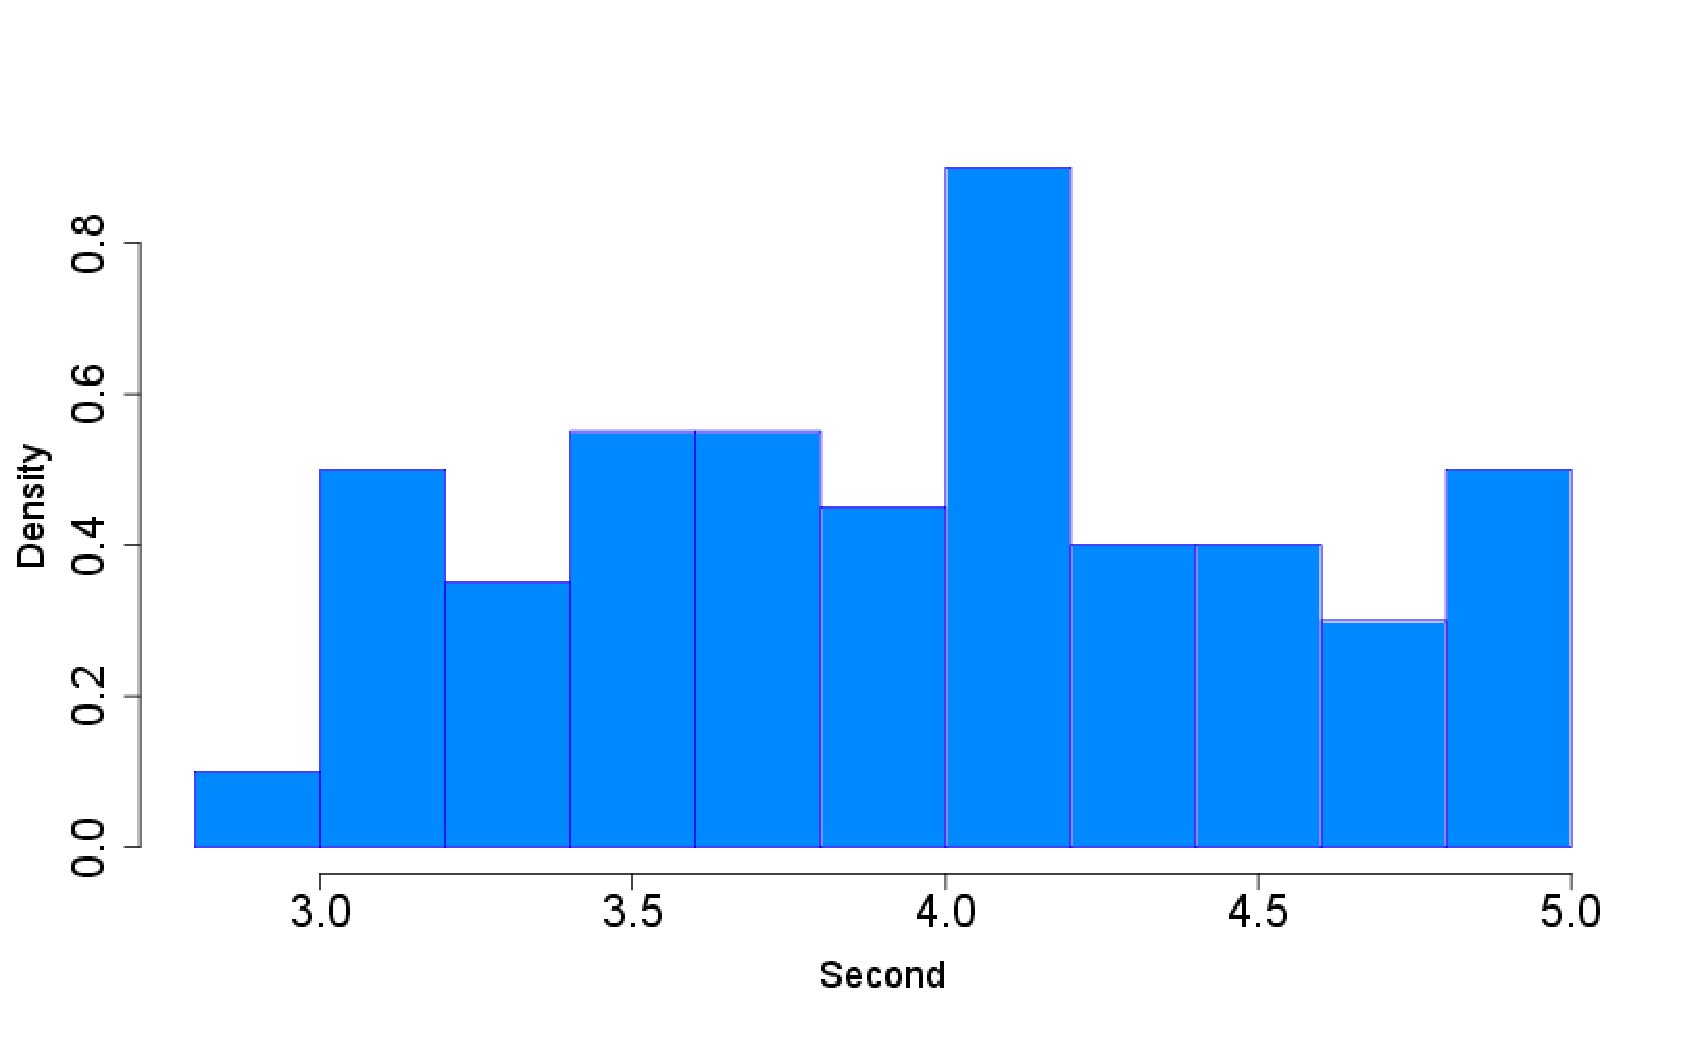
\includegraphics[keepaspectratio, width=80mm,height=40mm]{TotalTime.eps}
 \end{center}
 \caption{Total processing time}
 \label{TimeT}
\end{figure}

%6
\section{シミュレーション評価}
%事前実験で得られたデータを元に
%シミュレーション環境を構築

%参加型・無意識参加型のモデルを作成しセンサデータ取得率を比較
従来の参加型センシングによるセンシングデータ報告数において,提案する無意識参加型センシングの有効性を調べるためのシミュレーション実験を行う.
評価方法として,従来の参加型センシングにおけるセンシングデータ報告数とセンサデバイスが主体となる無意識参加型センシングでのセンシングデータ報告数を比較する.

\subsection{シミュレーション環境}
シミュレーション方法はミュレーションフレームワークであるScenargieとMultiAgentExtentionModuleを用いた.また地図サービスはOpenStreetMapを用いた.
図\ref{SimulationE}は今回使用するシミュレーションのマップであり,市街地を想定したマップに対して環境情報を定点観測するセンサデバイスを複数配置する.
図\ref{SimulationE}中の各センサにおける特徴はセンサ1が幹線道路クラスの道幅(25m),センサ2が主要道路クラスの道幅(20m),センサ3が道幅(15m),センサ4が小道(5m)の道幅に
設置してある.
図\ref{SimulationE}で使用したマップは愛知県の金山で格子状であり,道幅が均等でないところを選び使用した.
次にランダムに移動する参加者を想定したノードを配置し,Scenargieを用いてセンサデバイスと参加者の持つスマートフォンとの無線通信を想定したシミュレーションを行った.

\begin{figure}[tb]
\begin{minipage}[t]{1.0\columnwidth}
\CaptionType{table}
\caption{シミュレーションパラメータ}
%\ecaption{A table built by\\ Fig.\,\protect\ref{fig:left}.}
\label{tab:right}
\vskip1mm
\makebox[\textwidth][c]{\begin{tabular}[t]{lcr}\hline\hline
パラメータ項目&値\\\hline
フィールドサイズ&500×500[m]\\
参加者数&850\\
参加者の移動速度&1.5〜2.0[m/s]\\
センシングポイント数&4\\
シミュレーション時間&6000[s]\\
センシング依頼周期&600[s]\\
センシング依頼回数&10[回]\\
センシング範囲(無意識参加型)&半径30[m]\\\hline
\end{tabular}}
\end{minipage}
\end{figure}

\begin{figure}[b]
 \begin{center}
  \includegraphics[keepaspectratio, width=80mm,height=43mm]{Simulation_environment.eps}
 \end{center}
 \caption{Simulation environment}
 \label{SimulationE}
\end{figure}

\if0
\begin{figure*}[tb]
 \begin{center}
  \includegraphics[keepaspectratio, width=300mm,height=100mm]{Simulation_environment.eps}
 \end{center}
\caption{Simulation environment}
%\ecaption{Double column figure.}
\label{fig:double}
\end{figure*}
\fi

\subsection{想定するシナリオ}
表\ref{tab:right}は今回シミュレーションで行う際に使用したパラメータである.本シミュレーションでは,0.5km×0.5kmサイズのフィールド上を複数のセンシング参加者が1.5〜2.0m/sの速度でランダムに移動を行う.1.5〜2.0m/sは人間の通常歩行速度から算出している.参加者の数は850人としている.参加者の算出には政府統計の総合窓口(e-Stat)\cite{eStat}よりダウンロードした国勢調査(総務省統計局)の統計データに総務省の情報通信の現況・政策の動向からスマートフォン利用率約42\%\cite{General}を用いて算出した.フィールド上に,格子状に通行路が存在し,各地点にセンシングポイントが4つ存在している.センシングポイントでは物理センサにより温度や湿度,照度,音など環境情報を定点観測している事を想定する.
シミュレーションで行う参加型センシングのシナリオ及び無意識参加型センシングのシナリオを紹介する.

\subsubsection{参加型センシングシナリオ}
参加型センシングのシミュレーションでは格子状の通行にセンシングポイントを複数箇所設ける.センシング参加者に対して,依頼周期である600秒毎にセンシングポイントの各地点に対するセンシングを依頼する.クライアントはセンシング依頼周期毎に,フィールド上からランダムにセンシングポイントが選択されセンシング参加者にセンシングの依頼を行う.クライアントは最適な参加者を選択し,選択された参加者達はセンシングへの参加を決定した場合のみ,依頼を受けた地点に最短距離で移動を行い,センシングポイントにてセンシングされた情報を収集,報告し通常の動作に戻る.参加型センシングの場合,参加者に対してからなずしも依頼を受け入れ,行動してくれるとは限らいないため参加者のセンシングモチベーションなどによりセンシングを依頼しても行動してくれない可能性も考えられる.従って,参加者がセンシングの依頼を受け,行動しセンシングデータを報告するには参加者のモチベーションや報酬などに起因すると考えられる.そこで今回は,JMR生活総合研究所\cite{JMR}からイノベーション理論にある,イノベーター(2.5\%),アーリーアダプター(13.5\%)がセンシングに参加し依頼を承諾し行動,報告を行うものとし,約16\%がセンシングに参加するとした.%参加者の位置と以下の式に元ずいた行動を参加者は行う.
図\ref{ScenarioPa}にシミュレートするシナリオの概略図を示す.また以下に想定しているクライアントおよび参加者の振る舞いを示す.\\

\begin{description}
 \item[クライアント]\mbox{}
    \begin{itemize}
      \item センシング参加者の位置を事前に把握
      \item センシングポイントを指定
      \item センシング箇所へのタスク依頼を場合により報酬などと共に参加者に通知
      \item 各地点のセンシングデータを受信\\
    \end{itemize}
 \item[参加者]\mbox{}
    \begin{itemize}
      \item インターネットに接続可能なスマートフォンを携帯
      \item センシングに参加する場合は,指定のセンシングポイントまで移動しセンシングしたデータをクライアントに報告
    \end{itemize}
\end{description}

\begin{figure}[t]
 \begin{center}
  \includegraphics[keepaspectratio, width=80mm,height=40mm]{Participatory_sensing_case.eps}
 \end{center}
 \caption{Scenario of participatory sensing system}
 \label{ScenarioPa}
\end{figure}


\subsubsection{無意識参加型センシングシナリオ}
無意識参加型センシングのシミュレーションにおいても参加型センシングの環境と同様に格子状の通路にセンシングポイントを複数箇所設ける.無意識参加型センシングではクライアントからセンシング参加者に対して依頼するのではなくセンサポイントに設置されているセンサデバイスが参加者にセンシング及び報告を依頼する.したがってセンシング参加者は特に決められた動きをする事なく自由に行動する.参加者が偶然センシングポイントに近づき,センシング可能範囲内である半径30m以内に侵入し範囲内に4秒以上滞在した場合,自動的にセンシングを開始しクライアントへ報告を行う.センシング可能範囲内の30mはiBeacon及びBLEアドバタイズの理論値を用いて設定している.また事前実験により得られたセンシング処理時間を用いて滞在時間を算出している.図\ref{ScenarioUn}にシミュレートするシナリオ概要図を示す.また以下に想定しているクライアントおよび参加者,センサデバイスの振る舞いを示す.\\%センシング参加者は自由に行動をし,センシングポイントに偶然近づいた場合,センシングポイントに設置させているセンサデバイスが参加者にセンシングの依頼とクライアントへの報告を依頼する.以下に想定しているクライアント,参加者,センサデバイスの振る舞いを示す.¥¥


\begin{description}
 \item[クライアント]\mbox{}
    \begin{itemize}
      \item センシング参加者の位置を事前に把握不要
      \item 各地点のセンシングデータを受信\\
    \end{itemize}
 \item[参加者]\mbox{}
    \begin{itemize}
      \item インターネットに接続可能なスマートフォンを携帯
      \item 参加者はセンシングポイントの場所を意識不要
      \item センシングポイントの近隣に存在した場合、バックグラウンドでセンシング情報を収集しクライアントに報告\\
    \end{itemize}
 \item[センサデバイス]\mbox{}
    \begin{itemize}
      \item 近隣の参加者に対してセンシングを依頼
      \item 近隣の参加者にスマートフォンの回線を用いてセンシング情報の報告を依頼
    \end{itemize}
\end{description}


\begin{figure}[t]
 \begin{center}
  \includegraphics[keepaspectratio, width=80mm,height=40mm]{Unconscious_participatory_sensing_case.eps}
 \end{center}
 \caption{Scenario of unconscious participatory sensing system}
 \label{ScenarioUn}
\end{figure}


シミュレーションを行う参加型センシングと無意識参加型センシングの想定するシナリオを以下に示す.
\newpage
\subsection{シミュレーション結果}
シミュレーションの結果を図¥ref{Result}に示す.参加型センシングの場合はセンサ1〜3はほぼ同じ量のセンシングデータの報告があり,僻地で道幅が狭いセンサ4のみ,報告数が少ない結果となった.無意識参加型センシングの場合の場合は,道幅に大きさによって報告数が違う事が確認できた.道幅の一番大きな通り付近に設置してあるセンサ1が一番多く報告され,道幅が小さくなるにつれて報告数が減少している.従って,無意識参加型センシングは道幅や人通りの多さによって報告数が異なるという特徴が確認できた.つまり,道幅や人通りの大きい場所付近にセンサが設置してある場合には無意識参加型センシングの方がより多くのデータが収集できる事が確認できた.

シミュレーション結果は参加型センシングの場合,各センシングポイントでほぼ均等にデータの取得が可能
無意識参加型センシングの場合,道幅の広い道や交差点など人通りの多い付近のセンシングポイントでは参加型センシング
よりも多くデータ収集する事が可能であるが,人通りの少ない場所ではセンシングポイントに参加者が移動しないためデータ収集量が少なくなる.
従って,僻地や人通りの少ない場所においてセンシングポイントが存在した場合,参加型センシングの方がセンシングデータの多く収集可能であり,人通りの少ない場所においてセンシング情報を収集場合には参加型センシング方が有効である事が確認できた.一方で,大通に近いセンシングポイントや人通りが多い場所でのセンシングポイントでは無意識型センシングにおいてセンシング情報が多く収集できる事が確認できた.

\begin{figure}[t]
 \begin{center}
  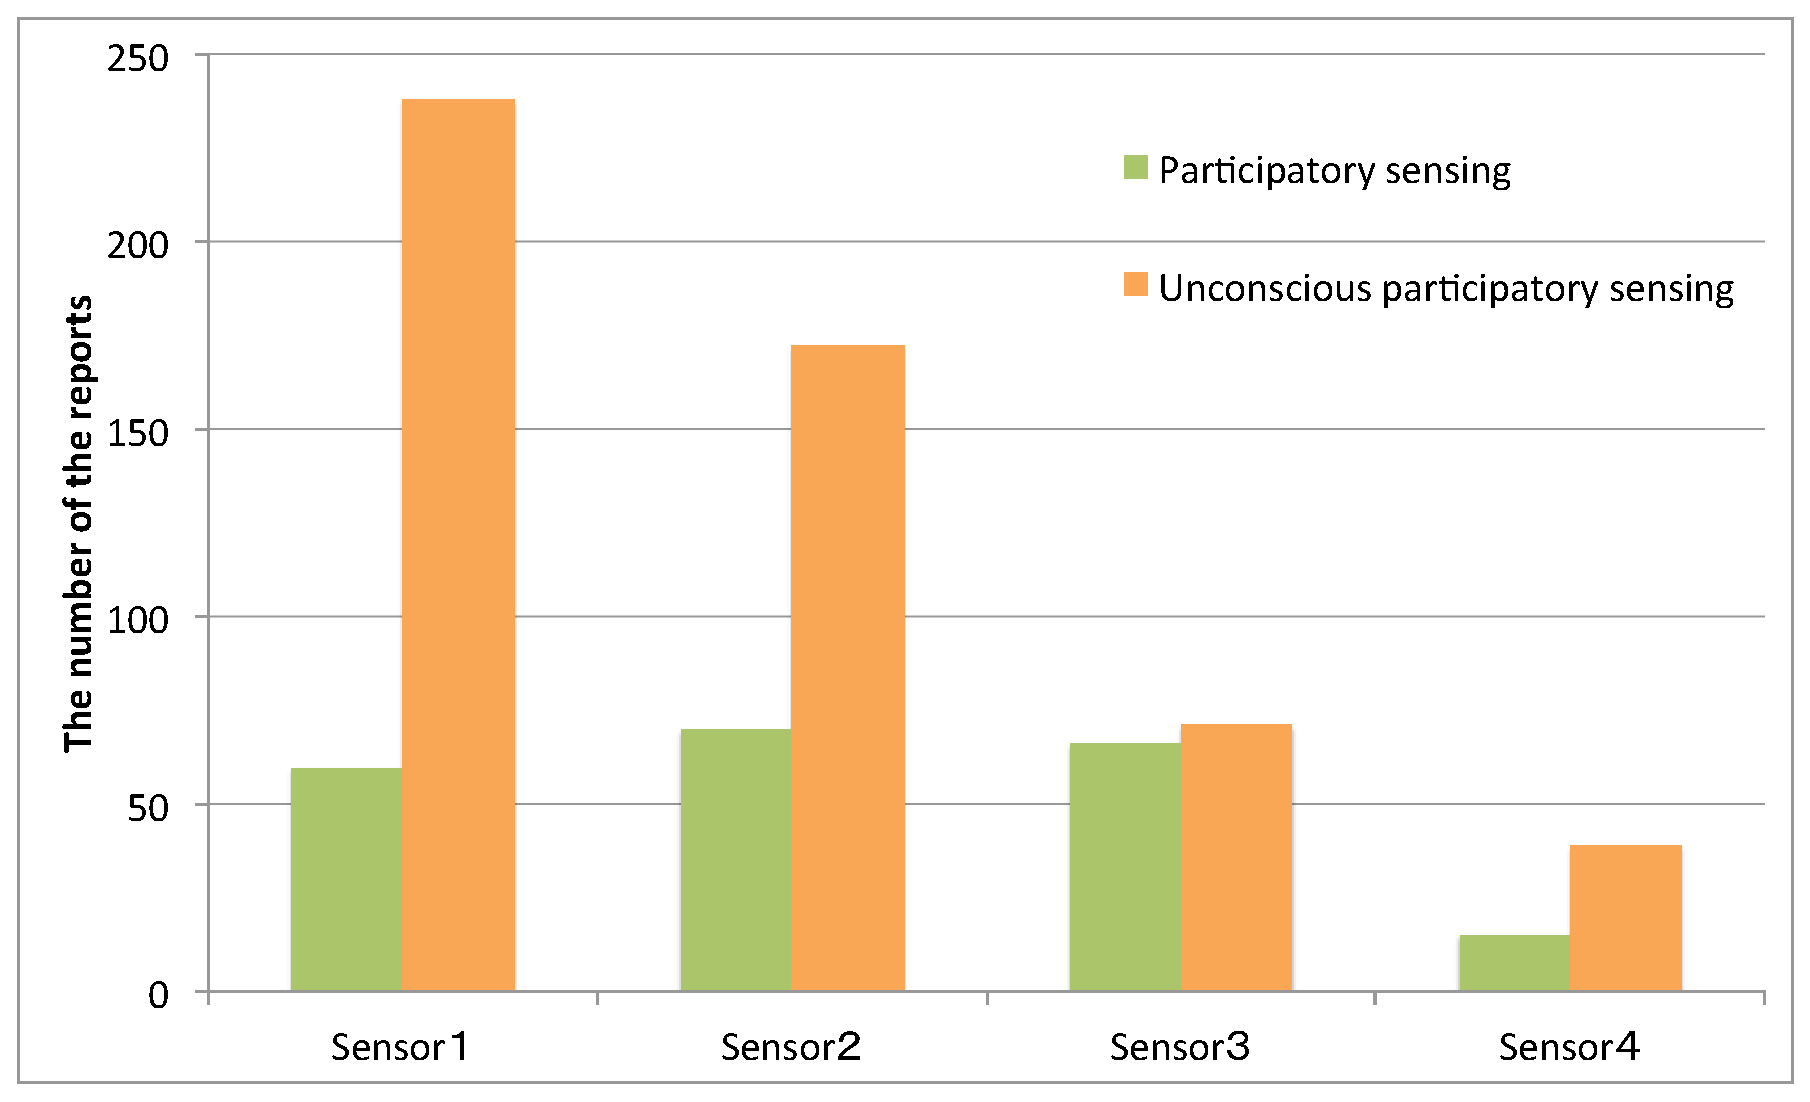
\includegraphics[keepaspectratio, width=80mm,height=43mm]{Result.eps}
 \end{center}
 \caption{Comparison of the number of the data reports}
 \label{Result}
\end{figure}

\section{まとめ}
本研究では,一般的な参加型センシングと無意識型センシングにおいてそれぞれシナリオを作成し,シミュレーションを行った.
それぞれの手法でセンシングポイントを設け,参加者を通じてセンシングデータの報告量について評価を行い,無意識型センシングの
特徴をシミュレーションにより確認することができた.シミュレーション結果より,無意識型センシングを評価した結果,すべてのセンシングポイントで参加型センシングより優れている訳ではなく,人通りの多い場所付近のセンシングポイントの場合,参加型センシングより多くのセンシングデータ収集できることが確認できた.従って,無意識参加型センシングにおいては人通りの多い場所や大通と行った道幅が広い場所付近でのセンシングデータ収集が参加型センシングよりも優れているという特徴が確認できた.今後はシミュレーションのシナリオの改善を行い,参加者の心理的な状態やセンシングポイントまでの距離や報酬などによって生じる行動の変化をシミュレーションによって実現し,より現実世界に近い環境下で評価実験を行っていきたい.


\label{config}

ファイルは次のようになる.下線部は投稿時に省略可能なもの.またトランザク
ション特有コマンドについては \ref{sig}~節を参照されたい.

4.1
\subsection{オプション・スタイル}

\label{option} \|\documentclass{ipsj}|のオプション\footnote{研究会用のオ

4.2
\subsection{表題・著者名等}

表題,著者名とその所属,および概要を前述のコマンドや環境により{\bf 和文と
英文の双方について}定義した後,\|\maketitle| によって出力する.

4.2.1
\subsubsection{表題}

表題は,\|\title| および \|\etitle| で定義した表題はセンタリングされる.
文字数の多いものについては,適宜 \|\\| を挿入して改行する.

4.2.2
\subsubsection{著者名・所属}

4.2.3
\subsubsection{概要}

和文の概要は \|abstract| 環境の中に,

4.2.4
\subsubsection{キーワード}

%英文の概要は \|ekeyword| 環境の中に,それぞれ1\UTF{FF5E}5語記述する.

%4.3
%\subsection{本文}

%4.3.1
%\subsubsection{見出し}

%4.3.2
%\subsubsection{行送り}


%4.3.3
%\subsubsection{フォントサイズ}

%4.3.4
%\subsubsection{句読点}

%句点には全角の「.」,読点には全角の「,」を用いる.ただし英文中や数式中
%で「.」や「,」を使う場合には,半角文字を使う.「.」や「,」は使わない.

%4.3.5
%\subsubsection{全角文字と半角文字}

%全角文字と半角文字の両方にある文字は次のように使い分ける.

%\begin{enumerate}
%\item 括弧は全角の「(」と「)」を用いる.但し,英文の概要,図表見出し,
%書誌データでは半角の「(」と「)」を用いる.

%4.3.6
%\subsubsection{箇条書}

%箇条書に関する形式を特に定めていない.場合に応じて標準的な \|enumerate|,
%\|itemize|, \|description| の環境を用いてよい.

%4.3.7
%\subsubsection{脚注}

%脚注は \|\footnote| コマンドを使って書くと,ページ単位に\footnote{脚注の
%例.}や\footnote{二つめの脚注.}のような参照記号とともに脚注が生成される.

%4.3.8
%\subsubsection{OverfullとUnderfull}

%4.4
%\subsection{数式}\label{sec:Item}

%4.4.1
%\subsubsection{本文中の数式}

%本文中の数式は \|$| と \|$|, \|\(| と \|\)|, あるいは \|math| 環境のいず
%れで囲んでもよい.

%4.4.2
%\subsubsection{別組の数式}

%別組数式(displayed math)については \|$$| と \|$$| は使用せずに,\|\[| と
%\|\]| で囲むか,\|displaymath|, \|equation|, \|eqnarray| のいずれかの環
%境を用いる.これらは
%

%4.4.3
%\subsubsection{eqnarray環境}


%4.4.4
%\subsubsection{数式のフォント}

%4.5
%\subsection{図}

%\begin{figure*}[tb]
%\setbox0\vbox{\large
%\hbox{\|\begin{figure*}[t]|}
%\hbox{\quad \|<|図本体の指定\|>|}
%\hbox{\|\caption{<|和文見出し\|>}|}
%\hbox{\|\ecaption{<|英文見出し\|>}|}
%\hbox{\|\label{| $\ldots$ \|}|}
%\hbox{\|\end{figure*}|}}
%\centerline{\fbox{\hbox to.9\textwidth{\hss\box0\hss}}}
%\caption{2段幅の図}
%\ecaption{Double column figure.}
%\label{fig:double}
%\end{figure*}

%4.6
%\subsection{表}

%また,表の上に和文と英文の双方の見出しを, \|\caption|と \|\ecaption| で
%指定する.表の参照は \|\tabref{<|ラベル\|>}| を用いて行なう.

%\begin{table}[tb]
%\caption{表の例}
%\ecaption{An Example of Table.}
%\label{tab:example}
%\hbox to\hsize{\hfil
%\begin{tabular}{l|lll}\hline\hline
%& column1 & column2 & column3 \\\hline
%row1 &	item 1,1 & item 2,1 & ---\\
%row2 &	---      & item 2,2 & item 3,2 \\
%row3 &	item 1,3 & item 2,3 & item 3,3 \\
%row4 &	item 1,4 & item 2,4 & item 3,4 \\\hline
%\end{tabular}\hfil}
%\end{table}




%4.7
%\subsection{参考文献・謝辞}

%4.7.1
%\subsubsection{参考文献の参照}

%本文中で参考文献を参照する場合には%,%参考文献番号が文中の単語として使われ
%る場合と,そうでない参照とでは,使用する文字の大きさが異なる.前者は
%\|\Cite|により参照し,後者は
%\|\cite|により参照する.たとえば;
%\|\cite|を使用する.参照されたラベルは自動的にソートされ,
%\|[]|でそれぞれ区切られる.
%
%\begin{quote}
%文献 \|\cite{companion,okumura}| は \LaTeX の総合的な解説書である.
%\end{quote}
%
%と書くと;
%
%\begin{quote}
%文献\cite{companion,okumura}は \LaTeX の総合的な解説書である.
%\end{quote}
%
%が得られる.

%4.7.2
%\subsubsection{参考文献リスト}


%4.8
%\subsection{著者紹介}

%6
%\section{まとめ}

%論文の内容について,論文誌ジャーナル編集委員会で作成した「べからず集」を
%以下に示す.投稿前のチェックリストとして利用頂きたい.これ以外にも,査読
%者用,メタ査読者用の「べからず集」\cite{webpage2}も公開しているので,参
%照されたい.また,作文技術に関する \cite{book1, book2, book3, book4}のよ
%うな書籍も参考になる.

%5.1
%\subsection{書き方の基本}

%5.2
%\subsection{新規性と有効性を明確に示す}

%\begin{itemize}
% \item[$\Box$] 在来研究との関連,研究の動機,ねらい等が明確に説明されて
%	       いないのは再考を要する.
% \item[$\Box$] 既知/公知の技術が何であって,何を新しいアイデアとして提
%	       案しているのかが書かれていないのは再考を要する.
%\item[$\Box$] 十分な参考文献は新規性の主張に欠かせない.
% \item[$\Box$] 提案内容の説明が,概念的または抽象的な水準に終始していて,
%	       読者が提案内容を理解できない(それだけで新規性が感じられ
%	       ないもの)のは再考を要する.
% \item[$\Box$] 論文で提案した方法の有効性の主張がない,またはきわめて貧
%	       弱なのは再考を要する.
%\end{itemize}

%5.3
%\subsection{書き方に関する具体的な注意}

%5.4
%\subsection{参考文献}

%5.5
%\subsection{二重投稿}


%5.6
%\subsection{他の人に読んでもらう}


%5.7
%\subsection{その他}

%6
%\section{おわりに}

\begin{thebibliography}{10}

%\bibitem{latex}
%Lamport, L.: {\em A Document Preparation System \LaTeX User's Guide \&
%  Reference Manual}, Addison Wesley, Reading, Massachusetts (1986).
% (Cooke, E., et al.訳:文書処理システム \LaTeX,アスキー出版局
%  (1990)).

%\bibitem{total}
%伊藤和人: \LaTeX トータルガイド,秀和システムトレーディング (1991).
%\bibitem{nodera}
%野寺隆志:楽々 \LaTeX,共立出版 (1990).

\if0
\bibitem{okumura}
奥村晴彦:改訂第5版 \LaTeXe 美文書作成入門,
技術評論社(2010).

\bibitem{companion}
Goossens, M., Mittelbach, F. and Samarin, A.:
{\it The LaTeX Companion},
Addison Wesley, Reading, Massachusetts (1993).

\bibitem{book1}
木下是雄:
理科系の作文技術,
中公新書(1981).

\bibitem{book2}
Strunk W. J. and White E.B.:
{\it The Elements of Style, Forth Edition},
Longman (2000).

\bibitem{book3}
Blake G. and Bly R.W.:
{\it The Elements of Technical Writing},
Longman (1993).

\bibitem{book4}
Higham N.J.:
{\it Handbook of Writing for the Mathematical Sciences},
SIAM (1998).

\bibitem{webpage1}
情報処理学会論文誌ジャーナル編集委員会:
投稿者マニュアル(online),
\urlj{http://www.ipsj.or.jp/journal /submit/manual/j\_manual.html}
(2007.04.05).

\bibitem{webpage2}
情報処理学会論文誌ジャーナル編集委員会:
べからず集(online),
\urlj{http://www.ipsj.or.jp/journal/manual /bekarazu.html}
(2011.09.15).
\fi

%1
\bibitem{Viani}
F. Viani, P. Rocca, G. Oliveri, and A. Massa:
Pervasive remote sensing through WSNs, In Antennas and Propagation (EUCAP), 2012 6th European Conference on, pp. 49-50. IEEE, 2012.

%2
%\bibitem{Lane}
%N. D. Lane, S. B. Eisenman, M. Musolesi, E. Miluzzo, and A. T. Campbell:
%Urban sensing systems: opportunistic or participatory?,
%In Proceedings of the 9th Workshop on Mobile Computing Systems and Applications, HotMobile'08, pp. 11-16, 2008.

%3
\bibitem{Nicholas}
N. D. Lane, E. Miluzzo, H. Lu, D. Peebles, T. Choudhury, and A. T. Campbell:
A survey of mobile phone sensing,
IEEE Communications Magazine, Vol. 48, No. 9,
September 2010.

%4
%\bibitem{Mohan}
%P. Mohan, V. N. Padmanabhan, and R. Ramjee:
%Nericell: rich monitoring of road and traffic conditions using mobile smartphones,
%SenSys'08: Proceedings of the 6th ACM Conference on Embedded Network Sensor Systems,
%November 2008.

%5
\bibitem{Burke}
J. Burke, D. Estrin, M. Hansen, A. Parker, N. Ramanathan, S. Reddy, and M. B. Srivastava:
Participatory sensing, Mobile Device Centric Sensor Networks and Applications,
In Workshop on World-Sensor-Web (WSW),
pp. 117-134, 2006.

%6
%\bibitem{Wang}
%D. Wang, M. T. Amin, S. Li, T. Abdelzaher, L. Kaplan, S. Gu, C. Pan, H. Liu, C. C. Aggarwal, R. Ganti, X. Wang, P. Mohapatra, B. Szymanski, and H. Le:
%Using Humans as Sensors: An Estimation-theoretic Perspective,
%In
%IPSN'14 Proceedings of the 13th International Symposium on Information Processing in Sensor Networks,
%pp. 35-46, 2014.

%7
\bibitem{Niforatos}
%E. Niforatos, A. Vourvopoulos, M. Langheinrich, P. Campos, and A. Doria:
%Atmos: a hybrid crowdsourcing approach to weather estimation,
%UbiComp'14: Proceedings of the 2014 ACM International Joint Conference on Pervasive and Ubiquitous Computing,
%September 2014.

%8
\bibitem{Lam}
A. H. Lam, Y. Yuan, and D. Wang:
An occupant-participatory approach for thermal comfort enhancement and energy conservation in buildings, The 5th International Conference on Future Energy Systems (e-Energy'14), June 2014.

%9
%\bibitem{Budde}
%M. Budde, R. E. Masri, T. Riedel, and M. Beigl:
%Enabling Low-Cost Particulate Matter Measurement for Participatory Sensing Scenarios,
%In Proceedings of the 12th International Conference on Mobile and Ubiquitous Multimedia (MUM'13), December 2013.

%10
%\bibitem{Hull}
%B. Hull, V. Bychkovsky, Y. Zhang, K. Chen, M. Goraczko, A. Miu, E. Shih, H. Balakrishnan, and S. Madden:
%CarTel: a distributed mobile sensor computing system,
%In SenSys'06, pp. 125-138, 2006.

%11
%\bibitem{Zeiger}
%F. Zeiger and M. Huber:
%Demonstration abstract: participatory sensing enabled environmental monitoring in smart cities, The 13th International Symposium on Information Processing in Sensor Networks  (IPSN'14), April 2014.

%12
\bibitem{Shinohara}
篠原 雅貴,田島 誠也,中下 岬,近藤 亮磨,岩井 将行,"気体情報の時系列解析による集合施設の生活環境・活動状況推測システム",マルチメディア,分散協調とモバイルシンポジウム2014論文集,Vol.2014,pp.1892-1897,2014.
%巻,号,pp

%13
\bibitem{Li}
L. Li, Y. Zheng, and L. Zhang:
Demonstration abstract: PiMi air box: a cost-effective sensor for participatory indoor quality monitoring,
IPSN'14 Proceedings of the 13th International Symposium on Information Processing in Sensor Networks,
pp. 327-328, 2014.

%14
%\bibitem{Tomasic}
%A. Tomasic, J. Zimmerman, A. Steinfeld, and Y. Huang:
%Motivating Contribution in a Participatory Sensing System via Quid-Pro-Quo,
%In CSCW'14 Proceedings of the 17th ACM Conference on Computer Supported Cooperative Work \& Social Computing,
%pp. 979-988, 2014.

%15
%\bibitem{Zhang}
%D. Zhang, H. Xiong, L. Wang, and G. Chen:
%CrowdRecruiter: selecting participants for piggyback crowdsensing under probabilistic coverage constraint,
%UbiComp'14: Proceedings of the 2014 ACM International Joint Conference on Pervasive and Ubiquitous Computing,
%September 2014.

%16
\bibitem{Yoshitaka}
上山 芳隆 ,玉井 森彦 ,安本 慶一 ,"ユーザ参加型センシングにおけるゲーミフィケーションに基づくインセンティブ機構の提案",研究報告モバイルコンピューティングとユビキタス通信(MBL),Vol.66,No.12,pp.1-6,2013.
%巻,号,pp

%17
\bibitem{Demirbas}
M. Demirbas, M. A. Bayir, C. G. Akcora, Y. S. Yilmaz, and H. Ferhatosmanoglu:
Crowd-sourced sensing and collaboration using twitter,
WOWMOM'10 Proceedings of the 2010 IEEE International Symposium on A World of Wireless, Mobile and Multimedia Networks (WoWMoM),
pp. 1-9, 2010.

%18
\bibitem{Mizukami}
T. Mizukami, K. Naito, C. Doi, T. Nakagawa, K. Ohta, H. Inamura, T. Hishida, and T. Mizuno:
Fundamental Design for a Beacon Device Based Unconscious Participatory Sensing System,
International MultiConference of Engineers and Computer Scientists 2015, Vol. 2 2015.

%19
\bibitem{Scenargie}
Space-Time Engineering: Scenargie, [Online]. Available: http://www.spacetime-eng.com/en/products.html. Retrieved October 2015.

%20
\bibitem{iBeacon}
iBeacon for Developers,\\https://developer.apple.com/ibeacon/,
Retrieved October 2014.

%22
\bibitem{eStat}
e-Stat,\\http://www.e-stat.go.jp/SG1/estat/eStatTopPortal.do,
Retrieved October 2016.

%23
\bibitem{General}
総務省 情報通信の現況・政策の動向,\\
http://www.soumu.go.jp/johotsusintokei/\\
whitepaper/ja/h26/html/nc253120.html,
Retrieved October 2016.

%24
\bibitem{JMR}
JMR生活研究所 イノベーター理論,\\
http://www.jmrlsi.co.jp/knowledge/yougo/my02/my0219.html,
Retrieved October 2016.


\end{thebibliography}

\end{document}
